\documentclass[11pt,letter]{article}
\usepackage[utf8]{inputenc}
\usepackage{amsmath,amssymb,booktabs}
\usepackage[margin=2.3cm]{geometry}
\usepackage{xcolor,tcolorbox}
\usepackage{tikz,pgfplots}
\usepackage{listings}
\usepackage{hyperref}
\pgfplotsset{compat=1.18}
\hypersetup{hidelinks}
\definecolor{aggiemaroon}{RGB}{80,0,0}
\definecolor{teal}{RGB}{22,124,128}
\definecolor{gold}{RGB}{200,155,60}
\definecolor{lightteal}{RGB}{231,242,241}
\definecolor{lightgold}{RGB}{248,240,220}
\newcommand{\CFP}{C_{\mathrm{FP}}}
\newcommand{\CFN}{C_{\mathrm{FN}}}
\newtcolorbox{ideia}{colback=lightteal,colframe=teal,boxrule=0.7pt}
\newtcolorbox{atencao}{colback=lightgold,colframe=gold,boxrule=0.7pt}
\lstset{basicstyle=\ttfamily\small,frame=single,breaklines=true,showstringspaces=false}
\title{\textcolor{aggiemaroon}{The $\theta$ Threshold and Bayesian Probability}}
\author{DAEN 427 / ISEN 427 / ISEN 627 - Fall 2026\\[3ex]
        Alexander Abuabara}
\date{}
\begin{document}
\maketitle

\begin{ideia}
First, we define what would make a process problematic.
Next, we use data to calculate how likely it is that the problem exists.
Finally, we consider the costs of possible errors to decide whether we should
act.
\end{ideia}

The objective is to distinguish three quantities:
\[
\boxed{\theta_0\qquad q=P(\theta>\theta_0\mid D)\qquad \tau}
\]

\section{The true rate and its threshold}

Imagine a food manufacturing plant. We will use $\theta$ to represent the true
proportion of contaminated items produced by the line:
\[
\theta=\text{true contamination rate}.
\]
If $\theta=0.10$, approximately 10\% of the items would be contaminated in the
long run. The value of $\theta$ is unknown because we cannot test every item
produced in the past or every item that will be produced in the future.

Management considers a rate above 25\% unacceptable. This threshold is
\[
\theta_0=0.25.
\]
The adverse state is
\[
\theta>\theta_0,
\]
or, in this example,
\[
\theta>0.25.
\]

\begin{ideia}
The number $0.25$ defines when the true rate is considered too high. It does not
yet tell us the probability that the problem exists.
\end{ideia}

\subsection{An analogy}

A speed limit of 80 miles per hour defines what counts as speeding, but it does
not tell us the probability that a car is traveling above the limit. Similarly,
$\theta_0=0.25$ defines what counts as excessive contamination, but it does not
tell us the probability that $\theta$ is above that value.

\section{The prior, the data, and the posterior}

Before testing,
\[
\theta\sim\operatorname{Beta}(2,8).
\]
The plant tests 20 items and finds 8 contaminated items. There are 8 positive
results and 12 negative results. Using the Beta--Binomial update,
\[
\theta\mid D
\sim\operatorname{Beta}(2+8,8+12)
=\operatorname{Beta}(10,20).
\]
The symbol $D$ represents the observed data. The expression $\theta\mid D$
means the distribution of $\theta$ after considering the data.

The observed proportion is
\[
\frac{8}{20}=0.40,
\]
while the posterior mean is
\[
E(\theta\mid D)=\frac{10}{10+20}=0.3333.
\]

\begin{atencao}
The posterior mean of $0.3333$ does not directly answer the question of how
likely $\theta$ is to be greater than $0.25$. To answer that question, we must
consider the entire posterior distribution.
\end{atencao}

\section{The Bayesian probability $q$}

Because $\theta$ is unknown, we calculate
\[
q=P(\theta>0.25\mid D).
\]
This is the probability that the true contamination rate is greater than 25\%,
given the observed data.
\subsection{Graph of the posterior distribution}

\begin{figure}[ht]
\centering
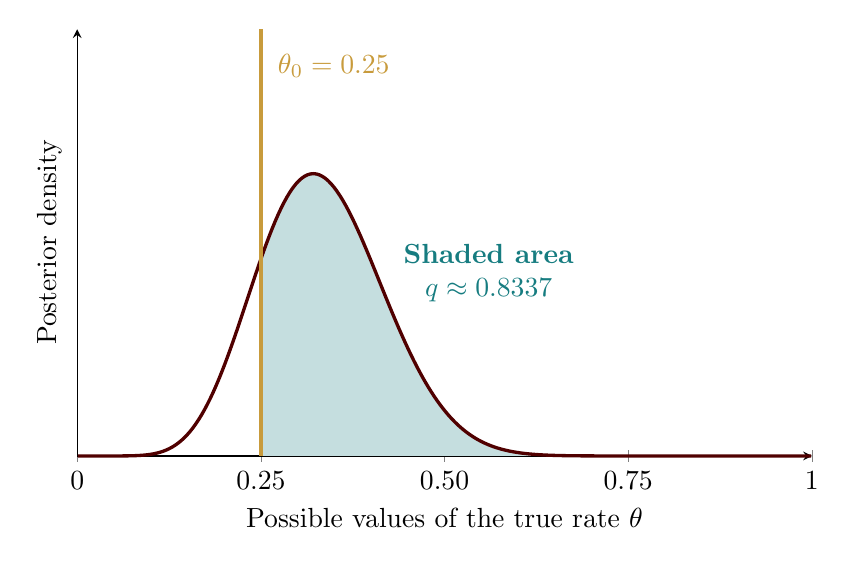
\begin{tikzpicture}
\begin{axis}[
  width=0.90\textwidth,
  height=7cm,
  xmin=0, xmax=1, ymin=0,
  axis lines=left,
  xlabel={Possible values of the true rate $\theta$},
  ylabel={Posterior density},
  xtick={0,0.25,0.5,0.75,1},
  xticklabels={$0$,$0.25$,$0.50$,$0.75$,$1$},
  ytick=\empty,
  samples=250,
  domain=0.001:0.999,
  clip=false
]
\addplot[draw=none,fill=teal!25,domain=0.25:0.999]
  {200300100*x^9*(1-x)^19} \closedcycle;
\addplot[very thick,aggiemaroon,domain=0.001:0.999]
  {200300100*x^9*(1-x)^19};
\addplot[very thick,gold] coordinates {(0.25,0) (0.25,7)};
\node[anchor=west,text=gold,font=\bfseries]
  at (axis cs:0.26,6.4) {$\theta_0=0.25$};
\node[align=center,text=teal,font=\bfseries]
  at (axis cs:0.56,3.0) {Shaded area\\$q\approx0.8337$};
\end{axis}
\end{tikzpicture}
\caption{Posterior $\operatorname{Beta}(10,20)$ distribution. The shaded
region represents $P(\theta>0.25\mid D)$.}
\end{figure}

The shaded area is
\[
q=P(\theta>0.25\mid D)\approx0.8337.
\]

\begin{ideia}
Given the model, the prior, and the test results, we assign an 83.37\%
posterior probability to the claim that the true contamination rate exceeds
25\%.
\end{ideia}

\section{How to calculate $q$}

The cumulative distribution function gives the probability that $\theta$ is to
the left of a specified value:
\[
F_{\operatorname{Beta}(10,20)}(0.25)
=P(\theta\leq0.25\mid D)
\approx0.166305.
\]
Because we want the area to the right,
\[
P(\theta>0.25\mid D)=1-P(\theta\leq0.25\mid D).
\]
Therefore,
\[
q=1-0.166305=0.833695\approx0.8337.
\]

\subsection{Calculation in R}

\begin{lstlisting}[language=R]
pbeta(
  0.25,
  shape1 = 10,
  shape2 = 20,
  lower.tail = FALSE
)
\end{lstlisting}

\subsection{Calculation in Python}

\begin{lstlisting}[language=Python]
from scipy.stats import beta
beta.sf(0.25, a=10, b=20)
\end{lstlisting}

In both cases, the approximate result is $0.8336951$.

\section{Why $\theta_0$ and $q$ are different}

\begin{center}
\begin{tabular}{lll}
\toprule
Quantity & Value & Meaning \\
\midrule
$\theta_0$ & $0.25$ & Threshold that defines an unacceptable rate \\
$q$ & $0.8337$ & Probability that $\theta$ is above $\theta_0$ \\
\bottomrule
\end{tabular}
\end{center}

First, we use $\theta_0$ to construct the event. Next, we calculate the
posterior probability of that event:
\[
\theta_0=0.25
\longrightarrow
\theta>0.25
\longrightarrow
q=P(\theta>0.25\mid D).
\]

\begin{atencao}
Comparing $0.8337$ directly with $0.25$ is not the decision rule.\\
To choose an action, we must compare $q$ with the action threshold $\tau$.
\end{atencao}
\section{The decision threshold $\tau$}

The decision depends on the consequences of two types of error.

\begin{center}
\begin{tabular}{p{3.8cm}p{4.8cm}p{4.8cm}}
\toprule
Decision & Rate is truly high & Rate is not high \\
\midrule
Stop and sanitize
& Correct decision
& False positive: unnecessary shutdown \\
Continue production
& False negative: untreated problem
& Correct decision \\
\bottomrule
\end{tabular}
\end{center}

Suppose that
\[
\CFP=40{,}000
\qquad\text{and}\qquad
\CFN=120{,}000.
\]
The decision threshold is
\[
\tau
=\frac{\CFP}{\CFP+\CFN}
=\frac{40{,}000}{40{,}000+120{,}000}
=0.25.
\]
We now compare two probabilities:
\[
q=0.8337>\tau=0.25.
\]

\begin{ideia}
Because $q>\tau$, the Bayesian decision is to \textbf{stop and sanitize the
production line}.
\end{ideia}

\section{The coincidence of the two values equal to $0.25$}

In this example, $\theta_0$ and $\tau$ are both equal to $0.25$, but this is
only a numerical coincidence:
\[
\theta_0=0.25:
\quad
\text{When is the process rate considered excessive?}
\]
\[
\tau=0.25:
\quad
\text{How much posterior probability is required to act?}
\]

If the two types of error had equal costs,
\[
\tau=\frac{1}{1+1}=0.50,
\]
but the adverse state would still be defined as $\theta>0.25$.

If management changed the adverse state to $\theta>0.35$, then
\[
q_{0.35}=P(\theta>0.35\mid D)\approx0.4076.
\]
Because the costs did not change, $\tau$ would remain equal to $0.25$. Since
\[
0.4076>0.25,
\]
the decision would still be to stop and sanitize.

\begin{atencao}
Changing $\theta_0$ changes the event whose probability we calculate. Changing
the costs changes $\tau$. Neither change, by itself, changes the
$\operatorname{Beta}(10,20)$ posterior distribution.
\end{atencao}

\section{Summary of the reasoning}

\begin{enumerate}
  \item Define the state:
        \[
        \theta>\theta_0.
        \]

  \item Update the distribution:
        \[
        \theta\mid D\sim\operatorname{Beta}(10,20).
        \]

  \item Calculate the probability:
        \[
        q=P(\theta>\theta_0\mid D).
        \]

  \item Convert the costs into a threshold:
        \[
        \tau=\frac{\CFP}{\CFP+\CFN}.
        \]

  \item Compare:
        \[
        \text{if }q>\tau,\text{ choose the positive action.}
        \]
\end{enumerate}

\begin{ideia}
$\theta_0$ defines the problem, $q$ measures our
confidence that the problem exists,\\and $\tau$ determines when it is worthwhile
to act.
\end{ideia}

\section{Check your understanding}

\begin{enumerate}
  \item What does $\theta_0=0.25$ represent?
  \item What does $q=0.8337$ mean?
  \item Why do $q$ and $\theta_0$ not play the same role?
  \item With which quantity should $q$ be compared when choosing an action?
\end{enumerate}

\subsection*{Answers}

\begin{enumerate}
  \item It is the threshold that determines when the true rate is excessive.
  \item It is the posterior probability that $\theta$ exceeds $0.25$.
  \item Because $\theta_0$ defines an event, while $q$ measures the probability
        of that event.
  \item With $\tau$, the threshold derived from the costs.
\end{enumerate}

\end{document}
